\documentclass[tikz = true, float=false, crop=false, 11pt]{standalone}

\usepackage{../myrawtex}

\ifstandalone
\usepackage{xr-hyper} % Needed for external references
\externaldocument{"24_appendix"} 
\fi

\begin{document}

	
\ifstandalone
\tableofcontents %to be removed in main section
\newpage
\fi

\section{CI Formula Evolution}

\subsection{Example 1: Uniform Random Variable with 100\% CI}

	\subsubsection{Initial Setup} 
	
	Random Variable $x$ having uniform probability density function $f(x)$. 	
	
		\begin{tikzpicture}
		\draw [<->,thick] (0,4) node (yaxis) [above] {$f(x)$}
		|- (10,0) node (xaxis) [right] {$x$};
		\draw [fill=palepinky] (4,0) rectangle (8,2);
		\node [below] at (4,0) {$(\theta-1)$};
		\node [below] at (6,0) {$\theta$};
		\node [below] at (8,0) {$(\theta+1)$};
		\draw[dashed] (yaxis) |- (4,2);
		\node [left] at (0,2) {$\dfrac{1}{2}$};
		\node at (6,1) {Area=1};
		\end{tikzpicture}
	
	This simply means, the converge probability, 
	
		\begin{equation}\label{eq:1}
		Pr(\theta-1 \leq x \leq \theta+1) = 1  
		\end{equation}
	
	That is, the probability that $x$ could be within $\theta \pm 1$ is 1. 
	
	\subsubsection{CI construction using Pivotal Quantity}
	
	In equation \ref{eq:1}, by adding $-\theta$ to the inequalities, we get,	
	  \begin{align}
	    \nonumber Pr(-\theta + \theta-1 \leq -\theta + x \leq -\theta + \theta + 1) = 1 \\  
	    \nonumber Pr( -1 \leq x - \theta \leq 1) = 1  \\
	  \end{align}
	  
	Multiplying by $-1$, and adding $x$
	 
	  \begin{align}
	    \nonumber Pr(1 \geq -x + \theta \geq -1) = 1 \\
	    \nonumber Pr(x+1 \geq \theta \geq x-1) = 1 \\
	    Pr(x-1 \leq \theta \leq x+1) = 1 \label{eq:3}
	  \end{align}
	
	Thus while $x$ could take value only between $\theta \pm 1$ for given probability, Equation \ref{eq:3} states, $\theta$ could also be only within $x \pm 1$ for same probability\\.
	
	\subsubsection{Intuitive Proof}
	
	Suppose $x$ takes a left extreme value as below within bounds $\theta \pm 1$.  
	
		\begin{tikzpicture}
		\draw [<->,thick] (0,4) node (yaxis) [above] {$f(x)$}
		|- (10,0) node (xaxis) [right] {$x$};
		\draw [fill=palepinky] (4,0) rectangle (8,2);
		\node [below] at (4,0) {$(\theta-1)$};
		\node [below] at (8,0) {$(\theta+1)$};
		\node [below] at (6,0) {$\theta$};

		\draw[dashed] (yaxis) |- (4,2);
		\node [left] at (0,2) {$\dfrac{1}{2}$};
		\node at (6,1) {Area=1};		
		
		\draw[fill=red] (4,0) circle [radius=0.1];
		\node [above right] at (4.2,0) {$x_0$};
		
		\draw[fill=blue] (6,0) circle [radius=0.1];
		\node [above right] at (6,0) {$x_0 + 1$};
		\end{tikzpicture}
	
	Then, we could already see, $\theta$ is at $x_0 + 1$ still respecting the bounds $x \pm 1$. 
	
	Suppose $x$ takes a right extreme value as below within bounds $\theta \pm 1$.  
	
		\begin{tikzpicture}
		\draw [<->,thick] (0,4) node (yaxis) [above] {$f(x)$}
		|- (10,0) node (xaxis) [right] {$x$};
		\draw [fill=palepinky] (4,0) rectangle (8,2);
		\node [below] at (4,0) {$(\theta-1)$};
		\node [below] at (8,0) {$(\theta+1)$};
		\node [below] at (6,0) {$\theta$};
		
		\draw[dashed] (yaxis) |- (4,2);
		\node [left] at (0,2) {$\dfrac{1}{2}$};
		\node at (6,1) {Area=1};		
		
		
		\draw[fill=red] (8,0) circle [radius=0.1];
		\node [above right] at (8,0) {$x_0$};
		
		\draw[fill=blue] (6,0) circle [radius=0.1];
		\node [above right] at (6,0) {$x_0 - 1$};
		\end{tikzpicture}
	
	Then, we could already see, $\theta$ is at $x_0 - 1$ still respecting the bounds $x \pm 1$. 
	
	
	Thus, while $x$ could be only within $\theta \pm 1$, it is also valid to say, $\theta$ could vary only within $x \pm 1$.  
	
		\begin{align}
		Pr(\theta - 1 \leq x \leq \theta + 1) = Pr(x - 1 \leq \theta \leq x + 1) = 1
		\end{align}

\subsection{Example 1b: Uniform Random Variable with 90\% CI}
	
	\subsubsection{Initial Setup} 
	
		Random Variable $x$ having uniform probability density function $f(x)$. 	
		
		\begin{tikzpicture}
		\draw [<->,thick] (0,4) node (yaxis) [above] {$f(x)$}
		|- (10,0) node (xaxis) [right] {$x$};
		\draw [fill=palepinky] (4.2,0) rectangle (7.8,2);
		\node [below] at (4.2,0) {$(\theta-0.9)$};
		\node [below] at (6,0) {$\theta$};
		\node [below] at (7.8,0) {$(\theta+0.9)$};
		\draw[dashed] (yaxis) |- (4,2);
		\node [left] at (0,2) {$\dfrac{1}{2}$};
		\node at (6,1) {Area=0.9};		
		\end{tikzpicture}
		
		This simply means, the converge probability, 
		
		\begin{align}
		Pr(\theta-0.9 \leq x \leq \theta+0.9) = 0.9  
		\end{align}
		
		That is, the probability that $x$ could be within $\theta \pm 0.9$ is 0.9 or 90\%. 
	
	\subsubsection{CI construction using Pivotal Quantity}

		In equation $5$, by adding $-\theta$ to the inequalities, we get,

		\begin{align}
		\nonumber Pr(-\theta + \theta-0.9 \leq -\theta + x \leq -\theta + \theta + 0.9) = 0.9 \\  
		\nonumber Pr( -0.9 \leq x - \theta \leq 0.9) = 0.9  \\
		\end{align}
		
		Multiplying by $-1$, and adding $x$
	
		\begin{align}
		\nonumber Pr(0.9 \geq -x + \theta \geq -0.9) = 0.9 \\
		\nonumber Pr(x+0.9 \geq \theta \geq x-0.9) = 0.9 \\
		Pr(x-0.9 \leq \theta \leq x+0.9) = 0.9
		\end{align}

		Thus, while $x$ could take value only between $\theta \pm 0.9$ for given probability 0.9, above equation states, $\theta$ could also be only within $x \pm 0.9$ for same probability.

	\subsubsection{Intuitive Proof}

	Suppose $x$ takes a left extreme value as below within bounds $\theta \pm 0.9$.  
	
		\begin{tikzpicture}
		\draw [<->,thick] (0,4) node (yaxis) [above] {$f(x)$}
		|- (10,0) node (xaxis) [right] {$x$};
		\draw [fill=palepinky] (4.2,0) rectangle (7.8,2);
		\node [below] at (4.2,0) {$(\theta-0.9)$};
		\node [below] at (6,0) {$\theta$};
		\node [below] at (7.8,0) {$(\theta+0.9)$};
		
		\draw[dashed] (yaxis) |- (4,2);
		\node [left] at (0,2) {$\dfrac{1}{2}$};
		\node at (6,1) {Area=0.9};			
		
		\draw[fill=red] (4.2,0) circle [radius=0.1];
		\node [above right] at (4.4,0) {$x_0$};
		
		\draw[fill=blue] (6,0) circle [radius=0.1];
		\node [above right] at (6,0) {$x_0 + 0.9$};
		\end{tikzpicture}

	Then, we could already see, $\theta$ is at $x_0 + 0.9$ still respecting the bounds $x \pm 0.9$. 
	
	Simply put, when $x$ is at $x_0 = \theta - 0.9$, then it automatically implies, $\theta = x_0 + 0.9$
	
	Suppose $x$ takes a right extreme value as below within bounds $\theta \pm 1$.  
	
		\begin{tikzpicture}
		\draw [<->,thick] (0,4) node (yaxis) [above] {$f(x)$}
		|- (10,0) node (xaxis) [right] {$x$};
		\draw [fill=palepinky] (4.2,0) rectangle (7.8,2);
		\node [below] at (4.2,0) {$(\theta-0.9)$};
		\node [below] at (6,0) {$\theta$};
		\node [below] at (7.8,0) {$(\theta+0.9)$};
		
		\draw[dashed] (yaxis) |- (4,2);
		\node [left] at (0,2) {$\dfrac{1}{2}$};
		\node at (6,1) {Area=0.9};			
		
		\draw[fill=red] (7.8,0) circle [radius=0.1];
		\node [above right] at (7.8,0) {$x_0$};
		
		\draw[fill=blue] (6,0) circle [radius=0.1];
		\node [above right] at (6,0) {$x_0 - 0.9$};
		\end{tikzpicture}
		
		Then, we could already see, $\theta$ is at $x_0 - 0.9$ still respecting the bounds $x \pm 0.9$. \\
		
		
		Thus, while $x$ could be only within $\theta \pm 0.9$, it is also valid to say, $\theta$ could vary only within $x \pm 0.9$.  
		
		\begin{align}
		Pr(\theta - 0.9 \leq x \leq \theta + 0.9) = Pr(x - 0.9 \leq \theta \leq x + 0.9) = 0.9
		\end{align}

\subsection{Example 2: Uniform Random Variable with 100\% CI}

	\subsubsection{Initial Setup} 
		
		Random Variable $x$ having uniform probability density function  
		
			\begin{align}
			f(x)=\dfrac{1}{\theta} {\mathrm{\ \ for\ \ }}{\frac{1}{2}}\theta \le x \le {\frac{3}{2}}\theta
			\end{align}

		
		\begin{tikzpicture}
		\draw [<->,thick] (0,4) node (yaxis) [above] {$f(x)$}
		|- (10,0) node (xaxis) [right] {$x$};
		\draw [fill=palepinky] (4.2,0) rectangle (7.8,2);
		\node [below] at (4.2,0) {$\frac{1}{2}\theta$};
		\node [below] at (6,0) {$\theta$};
		\node [below] at (7.8,0) {$\frac{3}{2}\theta$};
		\draw[dashed] (yaxis) |- (4,2);
		\node [left] at (0,2) {$\dfrac{1}{\theta}$};
		\node at (6,1) {Area=1};		
		\end{tikzpicture}

		This simply means, the converge probability, 

			\begin{align}
			Pr\Big( \frac{1}{2}\theta \leq x \leq \frac{3}{2}\theta\Big) = 1  
			\end{align}
		
		That is, the probability that $x$ could be within $\theta \pm \frac{1}{2}\theta$ is 1
		
	\subsubsection{CI construction using Pivotal Quantity}
	
			Multiplying by 2 in the inequalities,
			
			$$
			Pr\Big( \theta \leq 2x \leq 3\theta\Big) = 1
			$$
			
			Dividing by $\theta$,..
			
			$$
			Pr\Big( 1 \leq \frac{2x}{\theta} \leq 3 \Big) = 1
			$$
			
			Dividing by x and inversing the inequalities, and again multiplying by 2..
			
			\begin{align}
			\nonumber Pr\Big( \frac{1}{x} \leq \frac{2}{\theta} \leq \frac{3}{x} \Big) = 1 \\			
			\nonumber Pr\Big( x \geq \frac{\theta}{2} \geq \frac{x}{3} \Big) = 1 \\	
			\nonumber Pr\Big( 2x \geq \theta \geq \frac{2x}{3} \Big) = 1			
			\end{align}
			
			which is same as 
			\begin{align}
			Pr\Big( \frac{2x}{3} \leq \theta \leq 2x \Big) = 1
			\end{align}

	\subsubsection{Intuitive Proof}
	
			Suppose $x$ takes a left extreme value as below within bounds $\theta \pm \dfrac{\theta}{2}$.  
			
			\begin{tikzpicture}
			\draw [<->,thick] (0,4) node (yaxis) [above] {$f(x)$}
			|- (10,0) node (xaxis) [right] {$x$};
			\draw [fill=palepinky] (4.2,0) rectangle (7.8,2);
			\node [below] at (4.2,0) {$\frac{1}{2}\theta$};
			\node [below] at (6,0) {$\theta$};
			\node [below] at (7.8,0) {$\frac{3}{2}\theta$};

			\draw[dashed] (yaxis) |- (4,2);
			\node [left] at (0,2) {$\dfrac{1}{\theta}$};
			\node at (6,1) {Area=1};
					
			\draw[fill=red] (4.2,0) circle [radius=0.1];
			\node [above right] at (4.4,0) {$x_0$};
			
			\draw[fill=blue] (6,0) circle [radius=0.1];
			\node [above right] at (6,0) {$2x_0$};
			\end{tikzpicture} \\

	
			When $x$ is at $x_0 = \dfrac{\theta}{2}$, then $\theta = 2x_0$ \\
		
			Suppose $x$ takes a right extreme value as below within bounds $\theta \pm \dfrac{\theta}{2}$.  	
			
			\begin{tikzpicture}
			\draw [<->,thick] (0,4) node (yaxis) [above] {$f(x)$}
			|- (10,0) node (xaxis) [right] {$x$};
			\draw [fill=palepinky] (4.2,0) rectangle (7.8,2);
			\node [below] at (4.2,0) {$\frac{1}{2}\theta$};
			\node [below] at (6,0) {$\theta$};
			\node [below] at (7.8,0) {$\frac{3}{2}\theta$};
			
			\draw[dashed] (yaxis) |- (4,2);
			\node [left] at (0,2) {$\dfrac{1}{\theta}$};
			\node at (6,1) {Area=1};
			
			\draw[fill=red] (7.8,0) circle [radius=0.1];
			\node [above right] at (7.8,0) {$x_0$};
			
			\draw[fill=blue] (6,0) circle [radius=0.1];
			\node [above right] at (6,0) {$\frac{2x_0}{3}$};
			\end{tikzpicture} \\	
			
			When $x$ is at $x_0 = \dfrac{3\theta}{2}$, then $\theta = \dfrac{2x_0}{3}$ \\	
			
			Thus, while $x$ could be only within $\theta \pm \dfrac{\theta}{2}$, it is also valid to say, $\theta$ could vary only within $\Big(\dfrac{2x}{3},2x\Big)$.  
		
			\begin{align}
			Pr\Big(\theta - \dfrac{\theta}{2} \leq x \leq \theta + \dfrac{\theta}{2}\Big) = Pr\Big(\dfrac{2x}{3} \leq \theta \leq 2x\Big) = 1
			\end{align}		
			
\subsection{Example 3: Normal Distribution with 95\% CI}

	\subsubsection{Initial Setup} 
	
		Random Variable $x$ having uniform probability density function  

		\begin{align}
		f(x)=\dfrac{1}{\sigma\sqrt{2\pi}}e^{-\frac{1}{2}\Big(\frac{X-\mu}{\sigma}\Big)^2}
		\end{align}	
		% respective normal function for tikz
		\pgfmathdeclarefunction{gauss}{3}{%
			\pgfmathparse{1/(#3*sqrt(2*pi))*exp(-((#1-#2)^2)/(2*#3^2))}%
		}		
		

		\begin{tikzpicture}
		%https://tex.stackexchange.com/questions/100022/plotting-normal-distribution-in-pgfplots
		%https://tex.stackexchange.com/questions/43610/plotting-bell-shaped-curve-in-tikz-pgf
		\begin{axis}[
		no markers, 
		domain=0:6, 
		samples=100,
		ymin=0,
		axis lines*=left, 
		xlabel=$x$,
		ylabel=$f(x)$,
		height=5cm, 
		width=12cm,
		xtick=\empty, 
		ytick=\empty,
		enlargelimits=false, 
		clip=false, 
		axis on top,
		grid = major,
		axis lines = middle
		]
		\def\mean{3}
		\def\sd{1}
		\def\cilow{\mean - 1.96*\sd}
		\def\cihigh{\mean + 1.96*\sd}
		\addplot [draw=none, fill=yellow!25, domain=\cilow:\cihigh] {gauss(x, \mean, \sd)} \closedcycle;
		\addplot [very thick,cyan!50!black] {gauss(x, \mean, \sd)};
		\pgfmathsetmacro\valueA{gauss(1,\mean,\sd)}
		
		\draw [gray] (axis cs:\cilow,0) -- (axis cs:\cilow,\valueA)
		(axis cs:\cihigh,0) -- (axis cs:\cihigh,\valueA);
		\draw [yshift=0.3cm, latex-latex](axis cs:\cilow, 0) -- node [above] {Area = $0.95$} (axis cs:\cihigh, 0);
		\node[below] at (axis cs:\cilow, 0)  {$\mu - 1.96\sigma$}; 
		\node[below] at (axis cs:\mean, 0)  {$\mu$}; 
		\node[below] at (axis cs:\cihigh, 0)  {$\mu + 1.96\sigma$}; 		
		\end{axis}		
		\end{tikzpicture}	\\
		
		This simply means, the converge probability,  
		
		\begin{align}
			Pr( \mu - 1.96\sigma \leq x \leq \mu + 1.96\sigma ) = 0.95 \label{eq:n1}
		\end{align}
		
		That is, the probability that $x$ could be within $\mu \pm 1.96\sigma$ is 0.95 or 95\% 
		
	\subsubsection{Why 1.96?}
	
		Let us standardize the distribution to standard normal distribution, $Z = \dfrac{X-\mu}{\sigma}$. \\ \\
		When $X = \mu + 1.96\sigma$, $Z = \dfrac{\mu + 1.96\sigma - \mu}{\sigma} = 1.96$ \\ \\
		When $X = \mu - 1.96\sigma$, $Z = \dfrac{\mu - 1.96\sigma - \mu}{\sigma} = -1.96$ \\ \\
		The transformed distribution would look like below.  \\
		
		\begin{tikzpicture}
		%https://tex.stackexchange.com/questions/100022/plotting-normal-distribution-in-pgfplots
		%https://tex.stackexchange.com/questions/43610/plotting-bell-shaped-curve-in-tikz-pgf
		\begin{axis}[
		no markers, 
		domain=-3:3, 
		samples=100,
		ymin=0,
		axis lines*=left, 
		xlabel=$z$,
		ylabel=$f(z)$,
		height=5cm, 
		width=12cm,
		xtick=\empty, 
		ytick=\empty,
		enlargelimits=false, 
		clip=false, 
		axis on top,
		grid = major,
		axis lines = middle
		]
		\def\mean{0}
		\def\sd{1}
		\def\cilow{\mean - 1.96*\sd}
		\def\cihigh{\mean + 1.96*\sd}
		\addplot [draw=none, fill=yellow!25, domain=\cilow:\cihigh] {gauss(x, \mean, \sd)} \closedcycle;
		\addplot [very thick,cyan!50!black] {gauss(x, \mean, \sd)};
		\pgfmathsetmacro\valueA{gauss(1.96,\mean,\sd)}
		
		\draw [gray] (axis cs:\cilow,0) -- (axis cs:\cilow,\valueA)
		(axis cs:\cihigh,0) -- (axis cs:\cihigh,\valueA);
		\draw [yshift=0.3cm, latex-latex](axis cs:\cilow, 0) -- node [above] {Area = $0.95$} (axis cs:\cihigh, 0);
		\node[below] at (axis cs:\cilow, 0)  {$- 1.96$}; 
		\node[below] at (axis cs:\mean, 0)  {$0$}; 
		\node[below] at (axis cs:\cihigh, 0)  {$1.96$}; 		
		\end{axis}		
		\end{tikzpicture}	\\	
		
		If we look at the Z table for $Z = 1.96$, we will find value as $0.975$				

			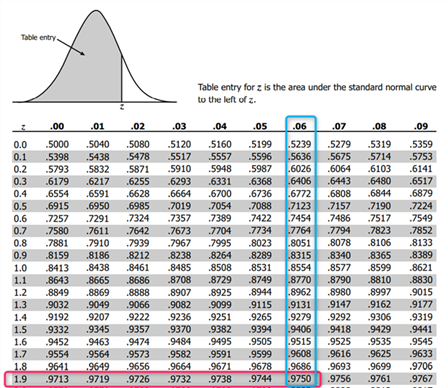
\includegraphics{../images/z196} \\ 
	
		If we look at the Z table for $Z = -1.96$, we will find value as $0.025$				
			
			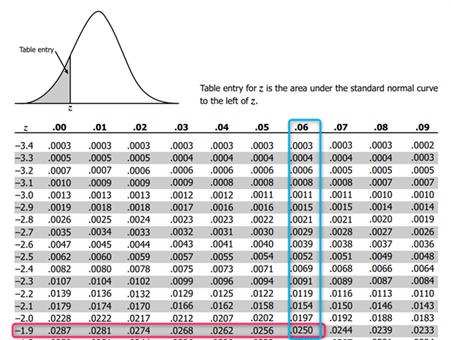
\includegraphics{../images/z1961} \\
			
		The area between $0.975$ and $0.025$ is $0.975-0.025 = 0.95$ or $95\%$. Thus, the value 1.96 was born. It depends on the area we are interested. Here, we were interested in 95\% area, so we get $Z = \pm 1.96$
		
		\paragraph{Note} \label{z_conv} The Z table might be left tailed as we just saw or also sometimes right tailed due to symmetrical nature of the curve. This realization is important because when we generalize CI, we will often take right tailed. I used the conventional left tailed table above just to state this explicitly as undoubting readers may miss this point. 
		
	\subsubsection{CI construction using Pivotal Quantity}
	
		From equation \ref{eq:n1}, adding $-\mu$ on both sides of inequalities, we get, 
		
			\begin{align}
			\nonumber Pr( -\mu + \mu - 1.96\sigma \leq x -\mu \leq -\mu + \mu + 1.96\sigma ) = 0.95 \\
			\nonumber Pr( - 1.96\sigma \leq x - \mu \leq  1.96\sigma ) = 0.95
			\end{align}
			
		And then adding $-x$
		
			\begin{align}
			\nonumber Pr( -x - 1.96\sigma \leq -x + x - \mu \leq  -x + 1.96\sigma ) = 0.95 \\
			\nonumber Pr( -x - 1.96\sigma \leq - \mu \leq  -x + 1.96\sigma ) = 0.95
			\end{align}
			
		Multiplying by $-1$
		
			\begin{align}
			\nonumber Pr( x + 1.96\sigma \geq \mu \geq  x - 1.96\sigma ) = 0.95 \\
			Pr( x - 1.96\sigma \leq \mu \leq x + 1.96\sigma)= 0.95 \label{eq:n9}
			\end{align}
						
	\subsubsection{Intuitive Proof}
		
		Suppose $x$ takes left extreme value within bounds $\mu \pm 1.96\sigma$. That is, $x_0 = \mu - 1.96\sigma$ Then, $\mu = x_0 + 1.96\sigma$ \\
			
		\begin{tikzpicture}
		%https://tex.stackexchange.com/questions/100022/plotting-normal-distribution-in-pgfplots
		%https://tex.stackexchange.com/questions/43610/plotting-bell-shaped-curve-in-tikz-pgf
		\begin{axis}[
		no markers, 
		domain=0:6, 
		samples=100,
		ymin=0,
		axis lines*=left, 
		xlabel=$x$,
		ylabel=$f(x)$,
		height=5cm, 
		width=12cm,
		xtick=\empty, 
		ytick=\empty,
		enlargelimits=false, 
		clip=false, 
		axis on top,
		grid = major,
		axis lines = middle
		]
		\def\mean{3}
		\def\sd{1}
		\def\cilow{\mean - 1.96*\sd}
		\def\cihigh{\mean + 1.96*\sd}
		\addplot [draw=none, fill=yellow!25, domain=\cilow:\cihigh] {gauss(x, \mean, \sd)} \closedcycle;
		\addplot [very thick,cyan!50!black] {gauss(x, \mean, \sd)};
		\pgfmathsetmacro\valueA{gauss(1,\mean,\sd)}
		
		\draw [gray] (axis cs:\cilow,0) -- (axis cs:\cilow,\valueA)
		(axis cs:\cihigh,0) -- (axis cs:\cihigh,\valueA);
		\draw [yshift=0.5cm, latex-latex](axis cs:\cilow, 0) -- node [above] {Area = $0.95$} (axis cs:\cihigh, 0);
		\node[below] at (axis cs:\cilow, 0)  {$\mu - 1.96\sigma$}; 
		\node[below] at (axis cs:\mean, 0)  {$\mu$}; 
		\node[below] at (axis cs:\cihigh, 0)  {$\mu + 1.96\sigma$}; 		
		
		% x left extreme value
		\draw[fill=red] (axis cs:\cilow,0) circle [radius=0.1cm];
		\node [above right] at (axis cs:\cilow,0) {$x_0$};
		\draw[fill=blue] (axis cs:\mean,0) circle [radius=0.1cm];
		\node [above right] at (axis cs:\mean,0) {$x_0 + 1.96\sigma$};				
		\end{axis}		
		\end{tikzpicture}	\\		
		
		Similarly, when $x_0 = \mu + 1.96\sigma$ then directly we could derive, $\mu = x_0 - 1.96\sigma$	
		
		\begin{tikzpicture}
		%https://tex.stackexchange.com/questions/100022/plotting-normal-distribution-in-pgfplots
		%https://tex.stackexchange.com/questions/43610/plotting-bell-shaped-curve-in-tikz-pgf
		\begin{axis}[
		no markers, 
		domain=0:6, 
		samples=100,
		ymin=0,
		axis lines*=left, 
		xlabel=$x$,
		ylabel=$f(x)$,
		height=5cm, 
		width=12cm,
		xtick=\empty, 
		ytick=\empty,
		enlargelimits=false, 
		clip=false, 
		axis on top,
		grid = major,
		axis lines = middle
		]
		\def\mean{3}
		\def\sd{1}
		\def\cilow{\mean - 1.96*\sd}
		\def\cihigh{\mean + 1.96*\sd}
		\addplot [draw=none, fill=yellow!25, domain=\cilow:\cihigh] {gauss(x, \mean, \sd)} \closedcycle;
		\addplot [very thick,cyan!50!black] {gauss(x, \mean, \sd)};
		\pgfmathsetmacro\valueA{gauss(1,\mean,\sd)}
		
		\draw [gray] (axis cs:\cilow,0) -- (axis cs:\cilow,\valueA)
		(axis cs:\cihigh,0) -- (axis cs:\cihigh,\valueA);
		\draw [yshift=0.5cm, latex-latex](axis cs:\cilow, 0) -- node [above] {Area = $0.95$} (axis cs:\cihigh, 0);
		\node[below] at (axis cs:\cilow, 0)  {$\mu - 1.96\sigma$}; 
		\node[below] at (axis cs:\mean, 0)  {$\mu$}; 
		\node[below] at (axis cs:\cihigh, 0)  {$\mu + 1.96\sigma$}; 		
		
		% x right extreme value
		\draw[fill=red] (axis cs:\cihigh,0) circle [radius=0.1cm];
		\node [above right] at (axis cs:\cihigh,0) {$x_0$};
		\draw[fill=blue] (axis cs:\mean,0) circle [radius=0.1cm];
		\node [above right] at (axis cs:\mean,0) {$x_0 - 1.96\sigma$};				
		\end{axis}		
		\end{tikzpicture}	\\			
		
		So, as $x_0$ varies from $\mu - 1.96\sigma$ to $\mu + 1.96\sigma$, implicitly, $\mu$ varies from $x_0 + 1.96\sigma$ to $x_0 - 1.96\sigma$. Thus, 
				
		\begin{align}
			Pr( \mu - 1.96\sigma \leq x \leq \mu + 1.96\sigma ) = Pr( x - 1.96\sigma \leq \mu \leq x + 1.96\sigma) = 0.95 \label{eq:n2}
		\end{align}
		
\section{CI for Sampling Distribution}

	\subsection{95\% CI as a Corollary}

	We already have seen, any sampling distribution for sample proportions or sample means, will approach normal distribution, with $\overline{X} \rightarrow \mu$ and $S \rightarrow \dfrac{\sigma}{\sqrt{n}}$, where $\mu, \sigma, n$ are population mean, population standard deviation, and sample size respectively, when respective conditions\footnote{$np \geq 10$ and $nq \geq 10$ for sample proportions, $n \geq 30$ for sample means} are met as per Central Limit theorem (CLT). Note each $x$ is a sample mean.
	
	We thus have a normal distribution like below representing sampling distribution.  \\
	
		\begin{tikzpicture}
		%https://tex.stackexchange.com/questions/100022/plotting-normal-distribution-in-pgfplots
		%https://tex.stackexchange.com/questions/43610/plotting-bell-shaped-curve-in-tikz-pgf
		\begin{axis}[
		no markers, 
		domain=0:6, 
		samples=100,
		ymin=0,
		axis lines*=left, 
		xlabel=$x$,
		ylabel=$f(x)$,
		height=5cm, 
		width=12cm,
		xtick=\empty, 
		ytick=\empty,
		enlargelimits=false, 
		clip=false, 
		axis on top,
		grid = major,
		axis lines = middle
		]
		\def\mean{3}
		\def\sd{1}
		\def\cilow{\mean - 1.96*\sd}
		\def\cihigh{\mean + 1.96*\sd}
		\addplot [draw=none, fill=yellow!25, domain=\cilow:\cihigh] {gauss(x, \mean, \sd)} \closedcycle;
		\addplot [very thick,cyan!50!black] {gauss(x, \mean, \sd)};
		\pgfmathsetmacro\valueA{gauss(1,\mean,\sd)}
		
		\draw [gray] (axis cs:\cilow,0) -- (axis cs:\cilow,\valueA)
		(axis cs:\cihigh,0) -- (axis cs:\cihigh,\valueA);
		\draw [yshift=0.3cm, latex-latex](axis cs:\cilow, 0) -- node [above] {Area = $0.95$} (axis cs:\cihigh, 0);
		\node[below] at (axis cs:\cilow, 0)  {$\overline{X} - 1.96S$}; 
		\node[below] at (axis cs:\mean, 0)  {$\overline{X}$}; 
		\node[below] at (axis cs:\cihigh, 0)  {$\overline{X} + 1.96S$}; 		
		\end{axis}		
		\end{tikzpicture}	\\
		
	Then, using equation \ref{eq:n2}, we have,
	
		\begin{align}
			\nonumber Pr( \overline{X} - 1.96S \leq x \leq \overline{X} + 1.96S ) = Pr( x - 1.96S \leq \overline{X} \leq x + 1.96S) = 0.95 \\
			 Pr( \mu - 1.96\frac{\sigma}{\sqrt{n}} \leq x \leq \mu + 1.96\frac{\sigma}{\sqrt{n}} ) = Pr( x - 1.96\frac{\sigma}{\sqrt{n}} \leq \mu \leq x + 1.96\frac{\sigma}{\sqrt{n}}) = 0.95 \label{eq:n3}
		\end{align}
		
	Thus, 95\% CI for a Sampling distribution would be $\Big(x \pm 1.96\frac{\sigma}{\sqrt{n}}\Big)$
	
	\subsection{Generalized CI}\label{sc:generalized-ci}
	
	As hinted in \ref{z_conv}, we will use a right tailed Z table for generalization. We already saw, at Z = -1.96, the area spanned would be 0.025. This could be written as 
	
	$$
	z_{0.025} = -1.96
	$$	
	
	Substituting in \ref{eq:n3}, we get,
		\begin{align}
		Pr( x - 1.96\frac{\sigma}{\sqrt{n}} \leq \mu \leq x + 1.96\frac{\sigma}{\sqrt{n}}) = 0.95 \nonumber \\
		Pr( x + z_{0.025}\frac{\sigma}{\sqrt{n}} \leq \mu \leq x - z_{0.025}\frac{\sigma}{\sqrt{n}}) = 0.95 \nonumber	
		\end{align}
	
	This is kind of counter intuitive. Additive term comes on the LHS. Though one would later discover, $z_{0.025}$ is negative, it could be better if this is not raising any confusion in first place. This is why we use right tailed Z table. 
	
	In case of right tailed Z table as below, note, at Z = 1.96, the area spanned is 0.025. Thus we could write it as 
	
	$$
	z_{0.025} = 1.96
	$$
	
		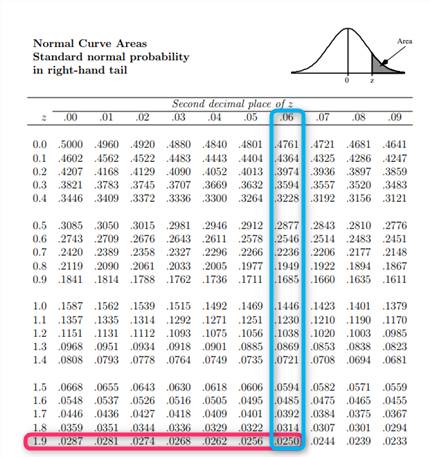
\includegraphics{../images/zr196} \\
		
	Substituting in \ref{eq:n3}, we get,
		\begin{align}
		Pr( x - 1.96\frac{\sigma}{\sqrt{n}} \leq \mu \leq x + 1.96\frac{\sigma}{\sqrt{n}}) = 0.95 \nonumber \\
		Pr( x - z_{0.025}\frac{\sigma}{\sqrt{n}} \leq \mu \leq x + z_{0.025}\frac{\sigma}{\sqrt{n}}) = 0.95 \nonumber	
		\end{align}
	
	This is good. 
	
	Let $\alpha$ be the desired significance level (which we will learn in hypothesis testing). In our case, it is 5\% or $\alpha = 0.05$. Thus, $1-\alpha = 0.95$ and $\frac{\alpha}{2} = 0.025$ 
	
	We could then rewrite above equation as, 
		\begin{align}
			Pr( x - z_{\frac{\alpha}{2}}\frac{\sigma}{\sqrt{n}} \leq \mu \leq x + z_{\frac{\alpha}{2}}\frac{\sigma}{\sqrt{n}}) = 1-\alpha \label{eq:n4}	
		\end{align}
		
	This is the generalized CI equation where $1-\alpha$ is called the {\bf confidence coefficient} and 
	$z_{\frac{\alpha}{2}}$ is called the {\bf critical value}
	
	\paragraph{Note} Confidence Interval CI indicates not an interval, where population mean is contained 95\% of time, but, if one continues to take many such samples and CI for each sample, then 95\% of those CIs would contain population mean. We do not know what those CIs are unless we know the population mean and take many such sample sets and their CIs. Once we have taken enough such sample sets (each sample set of size $n$) calculating CI each time, we could expect that 95\% of those CIs have population mean.
	
	
	\subsection{When $\sigma$ is known}
	In \ref{eq:n4}, we have population standard deviation $\sigma$ in both end points of the inequalities. Often population parameters are not known in reality. 
	So we have two cases: One when you are lucky enough to known $\sigma$ and another, you do not know. When you do know, still there are some more parts in play. For example, the more the samples are taken from population, the closer the resulting sampling distribution is to Normal (or Normal approximation is becoming better), so when do you say, sample size $n$ is good enough? This depends on various conditions. 
	
	
	\begin{enumerate}
		\item If we sample from population whose distribution is itself normal, then even small sample size {\boldmath{$n \geq 5$}}  would suffice because our sampling distribution easily approximates to Normal. Our current CI equation holds good.
		\begin{align}
			Pr( x - z_{\frac{\alpha}{2}}\frac{\sigma}{\sqrt{n}} \leq \mu \leq x + z_{\frac{\alpha}{2}}\frac{\sigma}{\sqrt{n}}) = 1-\alpha \nonumber
		\end{align}		
		\item If we sample from population whose distribution is not normal but symmetric, unimodal and of the continuous type, then as per Central limit theorem (CLT), sample size {\boldmath{$n \geq 30$}} should be adequate generally as this would result in sampling distribution becoming almost normal so our equation could still be approximately good. That is, 
			\begin{align}
			Pr( x - z_{\frac{\alpha}{2}}\frac{\sigma}{\sqrt{n}} \leq \mu \leq x + z_{\frac{\alpha}{2}}\frac{\sigma}{\sqrt{n}}) \approx 1-\alpha \label{eq:n5}	
			\end{align}
		\item If distribution is non normal and also highly skewed, even above approximation would not work. In that case, it would be safer to use certain nonparametric methods for finding a CI for the median of the distribution. 
	\end{enumerate}	

	\subsection{When $\sigma$ is not known}						
	This is often the case in reality. In this case, depending on certain conditions like above, we could use student's $t$ distribution\footnote{\url{http://pages.wustl.edu/montgomery/articles/2757}}. The $t$ distribution looks like normal, except the tails are bigger, and also depends on degrees of freedom (which usually is $n-1$). The proof is exhaustive, so we will take at face value for now (and prove in future if time permits)
	
	\begin{enumerate}
		\item If we sample from population whose distribution is itself normal, and
		if sample size {\boldmath{$n \leq 30$}}, then our CI equation would be,
		\begin{align}
			Pr( x - t_{\frac{\alpha}{2},(n-1)}\frac{s}{\sqrt{n}} \leq \mu \leq x + t_{\frac{\alpha}{2},(n-1)}\frac{s}{\sqrt{n}}) = 1-\alpha \label{eq:n6}
		\end{align}			
		where $t_{\frac{\alpha}{2},(n-1)}$ is the $t$ value for probability area $\frac{\alpha}{2}$, for degrees of freedom $(n-1)$ from corresponding right tailed $t$ table. 
		
		\item If we sample from population whose distribution is itself normal, and
		if sample size {\boldmath{$n > 30$}}, then our t distribution would already be almost equal to normal (and resulting sampling distribution would be normal) so we could use as below,
		\begin{align}
			Pr( x - z_{\frac{\alpha}{2}}\frac{s}{\sqrt{n}} \leq \mu \leq x + z_{\frac{\alpha}{2}}\frac{s}{\sqrt{n}}) = 1-\alpha \label{eq:n7}
		\end{align}	
		
		\item If we sample from population whose distribution is not normal but symmetric, unimodal and of the continuous type, and sample size {\boldmath{$n \leq 30$}}, we get approximate CI as below.
		\begin{align}
			Pr( x - t_{\frac{\alpha}{2},(n-1)}\frac{s}{\sqrt{n}} \leq \mu \leq x + t_{\frac{\alpha}{2},(n-1)}\frac{s}{\sqrt{n}}) \approx 1-\alpha \label{eq:n8}
		\end{align}	
		
		\item If distribution is non normal and also highly skewed, even above approximation would not work. In that case, it would be safer to use certain nonparametric methods for finding a CI for the median of the distribution. 
	\end{enumerate}

	\subsection{CI for difference between two means}
	
	This section is heavily inspired by \citet{robert2015}, and I have tried to articulate in my style to my understanding. Suppose that we are interested in comparing two approximately normal sampling distributions described by random variables $\overline{X} = N(\mu_{\overline{x}},\sigma_{\overline{x}}^2)$ and $\overline{Y} = N(\mu_{\overline{y}}, \sigma_{\overline{y}}^2)$, created from population distributions described by random variables $X(\mu_x,\sigma_x^2)$ and $Y(\mu_y,\sigma_y^2)$.	Note that $\overline{X}$ represents collection of sample means from sampled sets sampled from X and similarly for $\overline{Y}$. Since both $\overline{X}$ and $\overline{Y}$ are normally distributed, and assuming both are independent to each other, the distribution $W = \overline{X} - \overline{Y}$ would be again a normal distribution 
	$W(\mu_w,\sigma_w^2)$, where $\mu_w = \mu_{\overline{x}} - \mu_{\overline{y}}$ and $\sigma_w^2 = \sigma_{\overline{x}}^2 + \sigma_{\overline{y}}^2$ as proved in \ref{app_sc:001}
	
	
		\begin{tikzpicture}
		\begin{axis}[
		no markers, 
		domain=0:6, 
		samples=100,
		ymin=0,
		axis lines*=left, 
		xlabel=$w$,
		ylabel=$f(w)$,
		height=5cm, 
		width=12cm,
		xtick=\empty, 
		ytick=\empty,
		enlargelimits=false, 
		clip=false, 
		axis on top,
		grid = major,
		axis lines = middle
		]
		
		\def\mean{3}
		\def\sd{1}
		\def\cilow{\mean - 1.96*\sd}
		\def\cihigh{\mean + 1.96*\sd}
		\addplot [draw=none, fill=yellow!25, domain=\cilow:\cihigh] {gauss(x, \mean, \sd)} \closedcycle;
		\addplot [very thick,cyan!50!black] {gauss(x, 3, 1)};
		
		\pgfmathsetmacro\valueA{gauss(1,\mean,\sd)}
		\draw [gray] (axis cs:\cilow,0) -- (axis cs:\cilow,\valueA) (axis cs:\cihigh,0) -- (axis cs:\cihigh,\valueA);
	    \draw [yshift=0.3cm, latex-latex](axis cs:\cilow, 0) -- node [above] {Area = $1-\alpha$} (axis cs:\cihigh, 0);   

		\node[below] at (axis cs:\cilow, 0)  {$\mu_w - z_{\frac{\alpha}{2}}\sigma_w$}; 
		\node[below] at (axis cs:\mean, 0)  {$\mu_w$}; 
		\node[below] at (axis cs:\cihigh, 0)  {$\mu_w + z_{\frac{\alpha}{2}}\sigma_w$}; 
		
		
		\end{axis}
		\end{tikzpicture}	
	
	Since W is a normal distribution now, we have the confidence interval as follows directly following equation \ref{eq:n1}
	
	\begin{align}
		Pr( \mu - z_{\frac{\alpha}{2}}\sigma \leq x \leq \mu + z_{\frac{\alpha}{2}}\sigma ) = 1 - \alpha \nonumber \\
		Pr( \mu_w  - z_{\frac{\alpha}{2}}{\sigma_w} \leq W \leq \mu_w  + 	z_{\frac{\alpha}{2}}{\sigma_w}) = 1-\alpha \nonumber 	\\
		Pr(  -z_{\frac{\alpha}{2}}{\sigma_w} \leq W - \mu_w \leq  z_{\frac{\alpha}{2}}{\sigma_w}) = 1-\alpha \nonumber 	\\
		Pr(  -z_{\frac{\alpha}{2}} \leq \dfrac{W - \mu_w}{\sigma_w} \leq  	z_{\frac{\alpha}{2}}) = 1-\alpha \nonumber 
	\end{align}
	
	\begin{align}
			Pr(  -z_{\frac{\alpha}{2}} \leq \dfrac{W - \mu_w}{\sigma_w} \leq  	z_{\frac{\alpha}{2}}) = 1-\alpha \nonumber \\
			Pr\Big(  -z_{\frac{\alpha}{2}} \leq \dfrac{(\overline{X} - \overline{Y}) - (\mu_{\overline{x}} - \mu_{\overline{y}} )}{\sqrt{\sigma_{\overline{x}}^2 + \sigma_{\overline{y}}^2}} \leq  	z_{\frac{\alpha}{2}}\Big) = 1-\alpha \nonumber \\
			Pr\Bigg(  -z_{\frac{\alpha}{2}} \leq \dfrac{(\overline{X} - \overline{Y}) - (\mu_{\overline{x}} - \mu_{\overline{y}} )}{\sqrt{ {\frac{\sigma_x^2}{n}}   +  {\frac{\sigma_y^2}{m}}  }} \leq  	z_{\frac{\alpha}{2}}\Bigg) = 1-\alpha 	\label{eq:n12}
	\end{align}
	
	where $Z = \dfrac{W - \mu_w}{\sigma_w}$ would be the "standardized" normal distribution N(0,1), $n$ and $m$ are sample set sizes of $X(\mu_x,\sigma_x)$ and $Y(\mu_y,\sigma_y)$ respectively. 
	
	\subsubsection*{Assuming $\sigma$ unknown}
	
	Most of the times in reality, the population paramters are not known. So when the sample sizes $n,m$ are sufficiently large, we could use sample SDs ($s_{\overline{x}}, s_{\overline{y}}$) in place of ($\sigma_x,\sigma_y$). 
	
	
	\begin{align}
	Pr\Bigg(  -z_{\frac{\alpha}{2}} \leq \dfrac{(\overline{X} - \overline{Y}) - (\mu_{\overline{x}} - \mu_{\overline{y}} )}{\sqrt{ {\frac{s_{\overline{x}}^2}{n}}   +  {\frac{s_{\overline{y}}^2}{m}}  }} \leq  	z_{\frac{\alpha}{2}}\Bigg) \approx 1-\alpha  \nonumber			
	\end{align}	
	
	 And also rewriting, to find CI for ($\mu_{\overline{x}} - \mu_{\overline{y}}$), we get,
	 \begin{align}
	 Pr\Big(  (\overline{X} - \overline{Y}) - z_{\frac{\alpha}{2}}s_w \leq (\mu_{\overline{x}} - \mu_{\overline{y}}) \leq  	(\overline{X} - \overline{Y}) + z_{\frac{\alpha}{2}}s_w\Big) \approx 1-\alpha  			
	 \end{align}	
	
	where, $s_w = \sqrt{ {\frac{s_{\overline{x}}^2}{n}}   +  {\frac{s_{\overline{y}}^2}{m}}  }$, and $n,m$ are large. 
	
	\subsubsection*{When $n,m$ are small}
	
	We would then use student's $t$ distribution as suggested by {\textbf{\textit{Welch and Aspin}}}. The proof is currently beyond the scope so we take it at face value. 
	
	 \begin{align}
	Pr\Big(  (\overline{X} - \overline{Y}) - t_{(\frac{\alpha}{2},r)}s_w \leq (\mu_{\overline{x}} - \mu_{\overline{y}}) \leq  	(\overline{X} - \overline{Y}) + t_{(\frac{\alpha}{2},r)}s_w\Big) \approx 1-\alpha  \label{eq:n10}			
	\end{align}	
	
	where $r$ is degrees of freedom. Since two distributions are involved, calculating $r$ is complicated. It is given as follows: 
	
	\begin{align}
	r = \dfrac{  \Big(  \frac{s_x^2}{n} + \frac{s_y^2}{m}   \Big)^2  }{ \frac{1}{n-1}\Big(\frac{s_x^2}{n}\Big)^2 + \frac{1}{m-1}\Big(\frac{s_y^2}{m}\Big)^2  } \label{eq:n11}
	\end{align}	
	
	
	\subsubsection*{Protection when $\sigma_x = \sigma_y$}
	
	Since we do not know $\sigma_x,\sigma_y$, it might be that they are also equal. If they happen to be equal, r could be proven as below. 
	
	$$
	r = (n-1) + (m-1) = n + m - 2
	$$
	
	The equation \ref{eq:n11} protects in the sense that, the r value from that is lesser than above equation, so $t$ value is higher, or t distribution of wider variance assumed, thus being conservative. Some texts simply also take $r=min(n-1,m-1)$ as conservative approach. 
	
	\subsection*{A visual summary}
						\begin{tikzpicture}[node distance=2cm]
		\node (start) [startstop] {Start};
		\node (dec1) [decision, below of=start, yshift=-1cm] {$(\sigma_x,\sigma_y)$ known?};
		\node (dec2) [decision, right of=dec1, xshift=3cm] {$(n,m) > 30$?};
		\node (dec3) [decision, below of=dec2, yshift=-3cm, xshift=4cm] {$\sigma_x == \sigma_y$?};
		
		\node (pro1) [process, below of=dec1, yshift=-1cm] {Use $z$\\$\newline\sigma_w = \sqrt{\frac{\sigma_x^2}{n} + \frac{\sigma_y^2}{m}}$};
		\node (pro2) [process, below of=dec2, yshift=-1cm] {Use $z$\\$\newline\sigma_w = \sqrt{\frac{s_x^2}{n} + \frac{s_y^2}{m}}$};
		\node (pro4) [process, below of=pro2, yshift=-3cm, xshift=-1cm] {Use $t$\\$\newline r=\frac{ (\frac{s_x^2}{n} + \frac{s_y^2}{m})^2 }{ \frac{1}{n-1}(\frac{s_x^2}{n})^2 + \frac{1}{m-1}(\frac{s_y^2}{m})^2 }$\\$\newline\newline\sigma_w=\sqrt{\frac{s_x^2}{n} + \frac{s ^2}{m}}$};
		\node (pro3) [process, right of=pro4, xshift=3cm, yshift=-1cm] {Use $t$\\$\newline r=n+m-2$\\$\newline\sigma_w =\newline 
			S_p\sqrt{ \frac{ (n-1)s_x^2 +(m-1)s_y^2 }{ n+m-2 } }$\\$\newline S_p = \sqrt{\frac{1}{n} + \frac{1}{m}}$};
		
		
		\draw [arrow] (start) -- (dec1);
		\draw [arrow] (dec1) --  node[anchor=east] {yes} node[anchor=south, white, fill=black!30!green,xshift=-1.5cm, yshift=-0.20cm] {PR1} (pro1);
		\draw [arrow] (dec1) -- node[anchor=south, xshift=-0.5cm] {no} (dec2);
		\draw [arrow] (dec2) -- node[anchor=east] {yes} node[anchor=south, white, fill=black!30!green,xshift=-1.5cm, yshift=-0.20cm] {PR2} (pro2);
		\draw [arrow] (dec2) -| node[anchor=south, xshift=-2cm] {no} (dec3);
		\draw [arrow] (dec3) -- node[anchor=east] {yes} node[anchor=south, white, fill=black!30!green,xshift=-1.5cm, yshift=-0.18cm] {PR3} (pro3);
		\draw [arrow] (dec3) -| node[anchor=south, xshift=3cm] {no} node[anchor=south, xshift=1cm, yshift=-1cm] {Welch's t} node[anchor=south, white, fill=black!30!green, xshift=-1.5cm, yshift=-1.025cm] {PR4} (pro4);
		\end{tikzpicture}		
	
	
	\subsection{CI for difference between two proportions}	
	
    Suppose that we are interested in comparing two approximately normal sampling distributions described by random variables $ \displaystyle \frac{Y_1}{n_1} =  N\Big(p_1,\frac{p_1q_1}{n_1}\Big) $ and $ \displaystyle \frac{Y_2}{n_2} =  N\Big(p_2,\frac{p_2q_2}{n_2}\Big) $, created from population distributions which are Bernoulli distributions. 

	Note that $Y_1$ represents the sum of \textit{successes} in a sample set, and thus $\dfrac{Y_1}{n_1}$ represents sample proportions. For example, for any \textit{kth} sample set of $\dfrac{Y_1}{n_1}$, we calculate sample proportion statistic, $\dfrac{Y_{1k}}{n_1} = \dfrac {1}{n} \sum\limits_{i=1}^n Y_{1ki}$, where $Y_{1ki}$ is $i$th sample in $k$th sample set of sampling distribution described by $\dfrac{Y_1}{n_1}$. Similarly for $\dfrac{Y_2}{n_2}$
	
	We could then rewrite \ref{eq:n12} as below
	
	\begin{align}
	Pr\Bigg(  -z_{\frac{\alpha}{2}} \leq \dfrac{(\frac{Y_1}{n_1} - \frac{Y_2}{n_2}) - (p_1 - p_2) }{\sqrt{ {\frac{p_1q_1}{n_1}}   +  {\frac{p_2q_2}{n_2}}  }} \leq  	z_{\frac{\alpha}{2}}\Bigg) = 1-\alpha 
	\nonumber
	\end{align}    
	
	In case you are wondering about the parameters inside, say  $W = \dfrac{Y_1}{n_1} - \dfrac{Y_2}{n_2}$, then 
	
	$\mu_w = \mu_{y_1/n_1} - \mu_{y_2/n_2} = p_1 - p_2$  
	
	$\sigma_w^2 = \sigma_{y_1/n_1}^2 + \sigma_{y_2/n_2}^2 = \frac{p_1q_1}{n_1} + \frac{p_2q_2}{n_2} $
	$\therefore \sigma_w = \sqrt{\frac{p_1q_1}{n_1} + \frac{p_2q_2}{n_2}}$
	
	\subsubsection*{Assuming $\sigma$ unknown}
	
	Most of the times in reality, the population paramters are not known. So when the sample sizes $n,m$ are sufficiently large, we could use sample statistics ($\frac{\hat{p_1}\hat{q_1}}{n1},\frac{\hat{p_2}\hat{q_2}}{n2}$) in place of ($\frac{p_1q_1}{n1},\frac{p_2q_2}{n2}$). This results in further approximation of our confidence intervals. Thus when a sample is observed, we have statistics  
	
	$\hat{p_1} = \dfrac{y_1}{n_1} , \hat{q_1} = 1 - \dfrac{y_1}{n_1}$, 	 
	$\hat{p_2} = \dfrac{y_2}{n_2} , \hat{q_2} = 1 - \dfrac{y_2}{n_2}$, 	 	
	
	Thus we could rewrite further as,  
	
	\begin{align}
	Pr\Bigg(  -z_{\frac{\alpha}{2}} \leq \dfrac{(\hat{p_1} - \hat{p_2}) - (p_1 - p_2) }{\sqrt{ {\frac{\hat{p_1}\hat{q_1}}{n_1}}   +  {\frac{\hat{p_2}{\hat{q_2}}}{n_2}}  }} \leq  	z_{\frac{\alpha}{2}}\Bigg) \approx 1-\alpha \label{eq:n13} 
	\end{align}  	
	
	\subsubsection*{When $n,m$ are small}
	
	Currently I do not have an answer for this question and could not find online. Raised a ticket(?!) \href{https://stats.stackexchange.com/questions/369780/what-formula-for-confidence-intervals-for-difference-in-proportions-when-sample}{here}
	
	
	\ifstandalone
	\clearpage	
	\bibliography{../references} 
	\fi
	
\end{document}